% ==============================================================================
% 第 19 章：S-表达式之美 (Chapter 19: The Poetry of S-expressions)
% ==============================================================================

\chapter{S-表达式之美}
\label{sec:ch19_more_trees}

程序员常常利用树形数据结构来显著提升函数的执行性能。其中一种格外著名的树形结构是\term{二叉搜索树}（Binary Search Tree，简称 BST），因为它是快速存储和检索海量信息的经典方案。

\section{项目：二叉搜索树 }
\label{sec:19.5_bsts}

具体而言，我们讨论用于管理人事信息的二叉树。与家谱中的 \code{child} 结构体不同，二叉树由节点（node）构成：

\begin{lstlisting}[language=BSL]
(define-struct no-info [])
(define NONE (make-no-info))

(define-struct node [ssn name left right])

; 一个 BT（Binary Tree，二叉树）是下列之一：
; -- NONE
; -- (make-node Number Symbol BT BT)
\end{lstlisting}

相应的数据定义与家谱树非常相似：\code{NONE} 表示信息的缺失，每个 \code{node} 记录一个社会安全号（SSN，作为唯一的数字标识）、一个姓名以及另外两棵二叉树（左子树与右子树）。后两者类似于家谱中的父母，只是节点与其左右子树的关系不再基于血缘亲属，而是基于某种组织次序。

图~\ref{fig:119} 展示了如何用图形方式来理解这些树。在计算机科学中，树通常是倒着画的：根节点（root）在最顶端，树冠与树叶在最底部。每个圆圈对应一个节点，圆圈内的数字标明对应 \code{node} 结构体的 \code{ssn} 字段。在绘图中，\code{NONE} 通常被省略。

\begin{figure}[htbp]
  \centering
  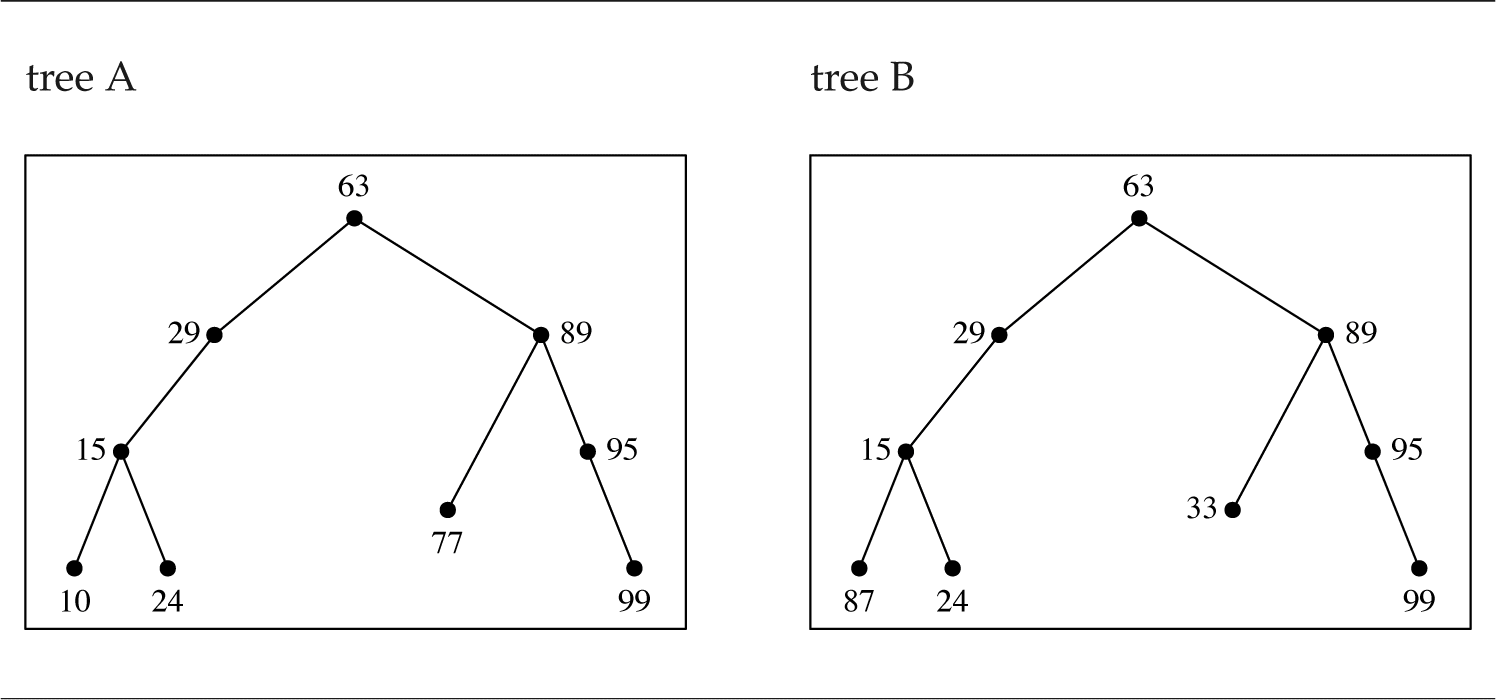
\includegraphics[width=0.85\textwidth]{images/00474.png}
  \caption{二叉搜索树与普通二叉树 (A binary search tree and a binary tree)}
  \label{fig:119}
\end{figure}

\begin{exercise}{绘制二叉树并设计 contains-bt?}{322}
按照图~\ref{fig:119} 的风格画出题目中给出的样本二叉树。然后设计函数 \code{contains-bt?}，判断给定的数字是否出现在某个给定的二叉树 \code{BT} 中。
\end{exercise}

\begin{exercise}{在二叉树中搜索指定社保号}{323}
设计函数 \code{search-bt}。该函数接收一个数字 \code{n} 与一棵二叉树 \code{BT}。若树中包含 \code{ssn} 为 \code{n} 的节点，则返回该节点的 \code{name} 字段值；否则返回 \code{\#false}。

\emph{提示：} 可以先调用 \code{contains-bt?} 检查整棵树，或者在每一步自然递归后使用 \code{boolean?} 检查递归结果。
\end{exercise}

如果我们从左向右读取图~\ref{fig:119} 中两棵树的所有数字，将得到两个不同的序列：
\begin{itemize}
  \item 树 A 的读取结果为：\code{(list 10 15 24 29 63 77 89 95 99)}
  \item 树 B 的读取结果为：\code{(list 15 24 10 29 95 63 89 77 99)}
\end{itemize}

树 A 的序列是严格升序排列的，而树 B 则不是。第一类具有有序性质的二叉树正是\term{二叉搜索树}（BST）。每一棵二叉搜索树都是二叉树，但并非每一棵二叉树都是二叉搜索树。更确切地说，我们可以表述区分二叉搜索树与普通二叉树的核心数据不变量：

\begin{notebox}[二叉搜索树不变量 (The BST Invariant)]
一棵 \term{BST} 是满足如下约束条件的 \code{BT}：
\begin{itemize}
  \item \code{NONE} 永远是一棵 BST；
  \item \code{(make-node ssn0 name0 L R)} 是一棵 BST，当且仅当：
  \begin{enumerate}
    \item \code{L} 是一棵 BST；
    \item \code{R} 是一棵 BST；
    \item \code{L} 中的所有 \code{ssn} 字段均\textbf{小于} \code{ssn0}；
    \item \code{R} 中的所有 \code{ssn} 字段均\textbf{大于} \code{ssn0}。
  \end{enumerate}
\end{itemize}
\end{notebox}

换言之，要验证一棵普通二叉树是否是二叉搜索树，我们必须检查所有子树中的数值，确保它们严格小于或大于当前节点的键值。这一不变量在构建数据时增加了一定约束，但在数据检索时将带来巨大的性能优势。

\begin{exercise}{二叉树的中序遍历 inorder}{324}
设计函数 \code{inorder}。该函数接收一棵二叉树，产生从左到右遍历树图时所见的所有 \code{ssn} 组成的列表。

\emph{提示：} 使用 \code{append} 拼接列表：
\begin{lstlisting}[language=BSL]
(append (list 1 2 3) (list 4) (list 5 6 7)) == (list 1 2 3 4 5 6 7)
\end{lstlisting}
思考：对一棵二叉搜索树执行 \code{inorder} 会产生什么样的列表？
\end{exercise}

在二叉搜索树中查找特定社保号的节点时，我们可以充分利用 BST 不变量。在普通二叉树中，为了确认某个数字是否存在，函数可能不得不遍历整棵树的每一个节点。相比之下，在二叉搜索树中，函数每访问一个节点，就可以果断\textbf{排除掉两棵子树中的一整棵}：

假设我们在如下样本 BST 中查找目标：
\begin{lstlisting}[language=BSL]
(make-node 66 'a L R)
\end{lstlisting}
如果目标是 66，查找成功。若目标小于 66（例如 63），我们只需聚焦于左子树 \code{L}，因为所有小于 66 的节点都在 \code{L} 中。反之，若目标是 99，我们可以完全忽略 \code{L}，直接在右子树 \code{R} 中查找。

\begin{exercise}{在二叉搜索树中高效查找 search-bst}{325}
设计函数 \code{search-bst}。该函数接收数字 \code{n} 与一棵二叉搜索树 \code{BST}。若树中包含 \code{ssn} 为 \code{n} 的节点，产生其 \code{name} 字段值；否则产生 \code{NONE}。函数组织结构必须利用 BST 不变量，使得执行的比较次数尽可能少。回顾第 189 题中有序列表的二分查找思想并进行对比！
\end{exercise}

构建一棵普通二叉树非常简单；但构建一棵二叉搜索树则需要缜密的逻辑。随意将两个 BST 和一个新数拼接，通常无法得到合法的 BST。

\begin{exercise}{向 BST 中插入节点 create-bst}{326}
设计函数 \code{create-bst}。该函数接收一个二叉搜索树 \code{B}、一个数字 \code{N} 以及一个符号 \code{S}。它生成一棵新的二叉搜索树，其内容与 \code{B} 相同，只是在恰当的 \code{NONE} 叶子位置插入了新节点：
\begin{lstlisting}[language=BSL]
(make-node N S NONE NONE)
\end{lstlisting}
设计完成后，在图~\ref{fig:119} 中的树 A 上测试该函数。
\end{exercise}

\begin{exercise}{从列表批量构建 BST}{327}
设计函数 \code{create-bst-from-list}。它接收一个由数与姓名组成的列表，通过反复调用 \code{create-bst} 从中构造出一棵完整的二叉搜索树。其函数签名如下：
\begin{lstlisting}[language=BSL]
; [List-of (list Number Symbol)] -> BST
\end{lstlisting}
使用该函数处理样本输入序列，验证是否能构造出图~\ref{fig:119} 中的树 A。如果你使用现有的列表折叠抽象（如 \code{foldr}），可能会得到一棵镜像“反转”的树，为什么？
\end{exercise}

\section{简化函数结构}
\label{sec:19.6_simplifying}

练习 317 展示了如何使用 \code{local} 来组织处理交织数据的多函数程序。当我们确定数据定义已经定型后，这种组织结构还能帮助我们大幅度精简代码。为了阐明这一点，我们展示如何系统性地化简练习 319 中 \code{substitute} 函数的实现。

图~\ref{fig:120} 展示了 \code{substitute} 的完整初始定义。该定义严格按照数据定义的要求，使用 \code{local} 声明了三个辅助函数，并附带了测试用例。

\begin{figure}[htbp]
  \centering
  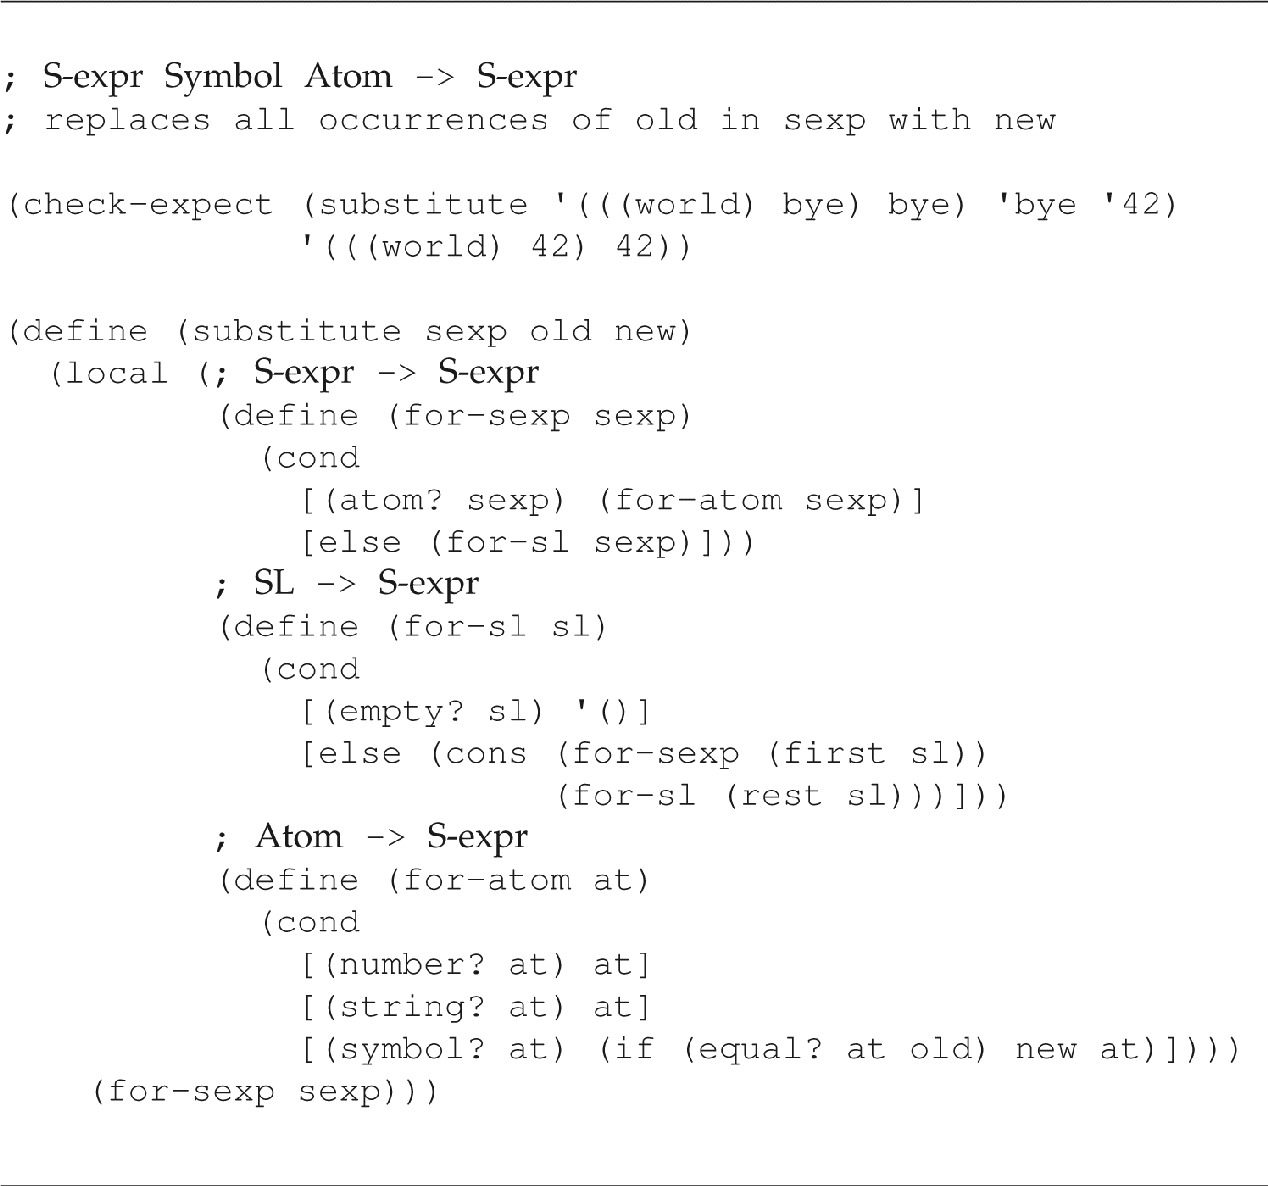
\includegraphics[width=0.85\textwidth]{images/00477.png}
  \caption{待化简的 S-表达式替换程序 (A program to be simplified)}
  \label{fig:120}
\end{figure}

\begin{exercise}{验证待化简程序}{328}
将图~\ref{fig:120} 复制到 DrRacket 中，补充充分的测试用例并运行。在阅读本节后续内容时，同步修改代码并重新运行测试套件，以验证每一步化简的等价性。
\end{exercise}

\textbf{第一步化简：利用现有抽象。} 鉴于 \code{SL} 本质上是 \code{S-expr} 的列表，我们可以使用高阶函数 \code{map} 极大简化 \code{for-sl}。原程序说明 \code{for-sexp} 作用于 \code{sl} 的每一项，使用 \code{map} 能更精准清晰地表达这一意图（见图~\ref{fig:121}）。

\begin{figure}[htbp]
  \centering
  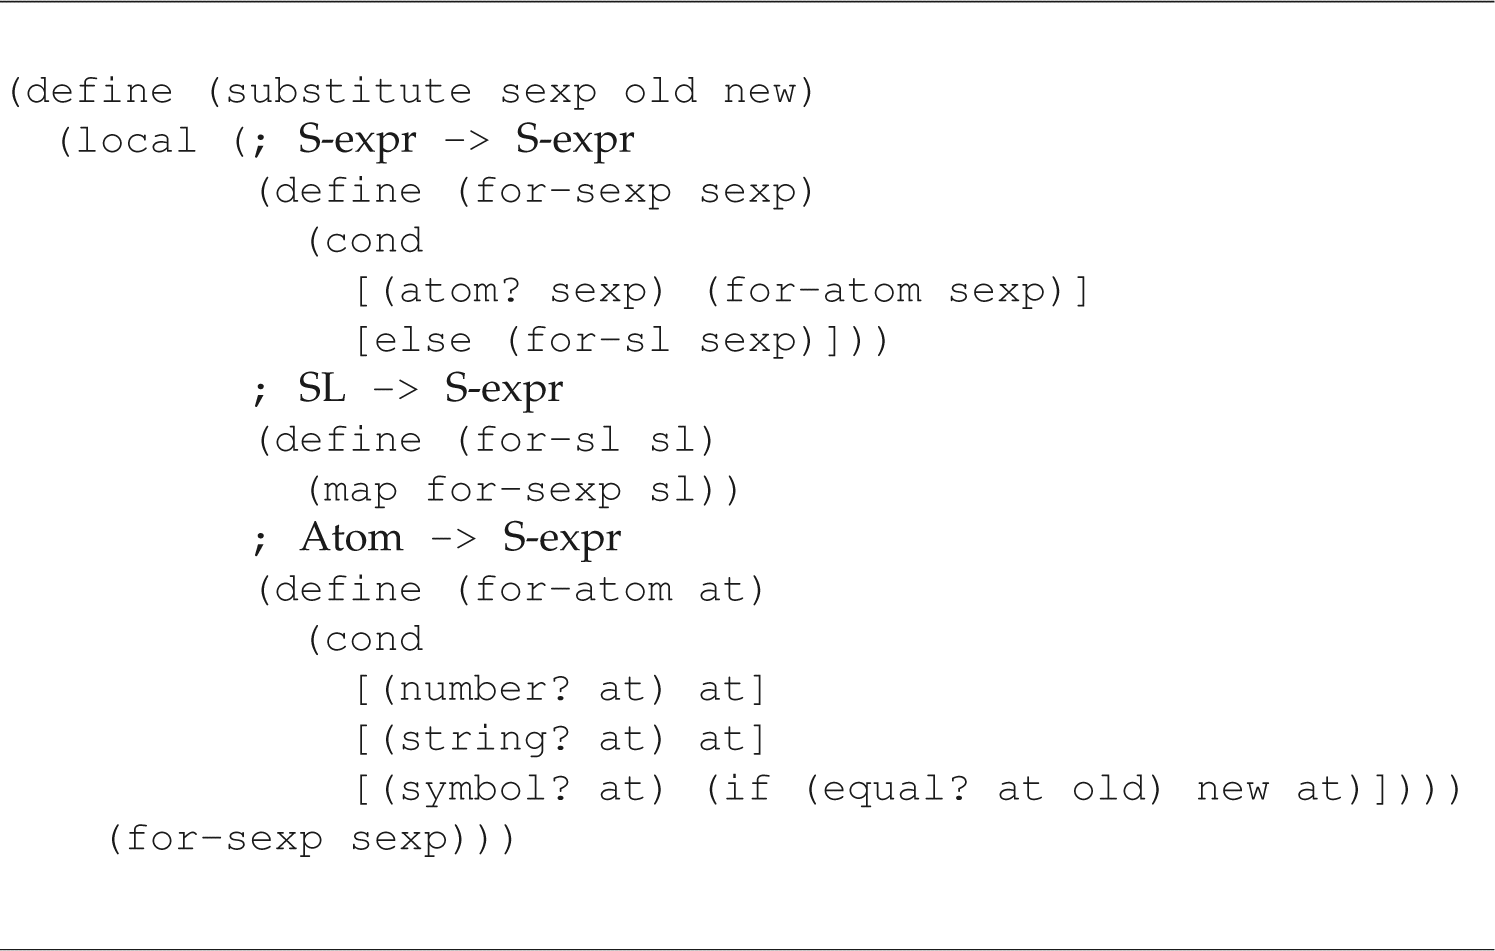
\includegraphics[width=0.85\textwidth]{images/00478.png}
  \caption{程序化简第一步：引入 map (Program simplification, step 1)}
  \label{fig:121}
\end{figure}

\textbf{第二步化简：通用相等比较。} 我们注意到 \code{equal?} 能够直接比较任意两个数据值。因此，第三个局部函数 \code{for-atom} 实际上可以精简为一行表达式。图~\ref{fig:122} 展示了这第二阶段的简化。

\begin{figure}[htbp]
  \centering
  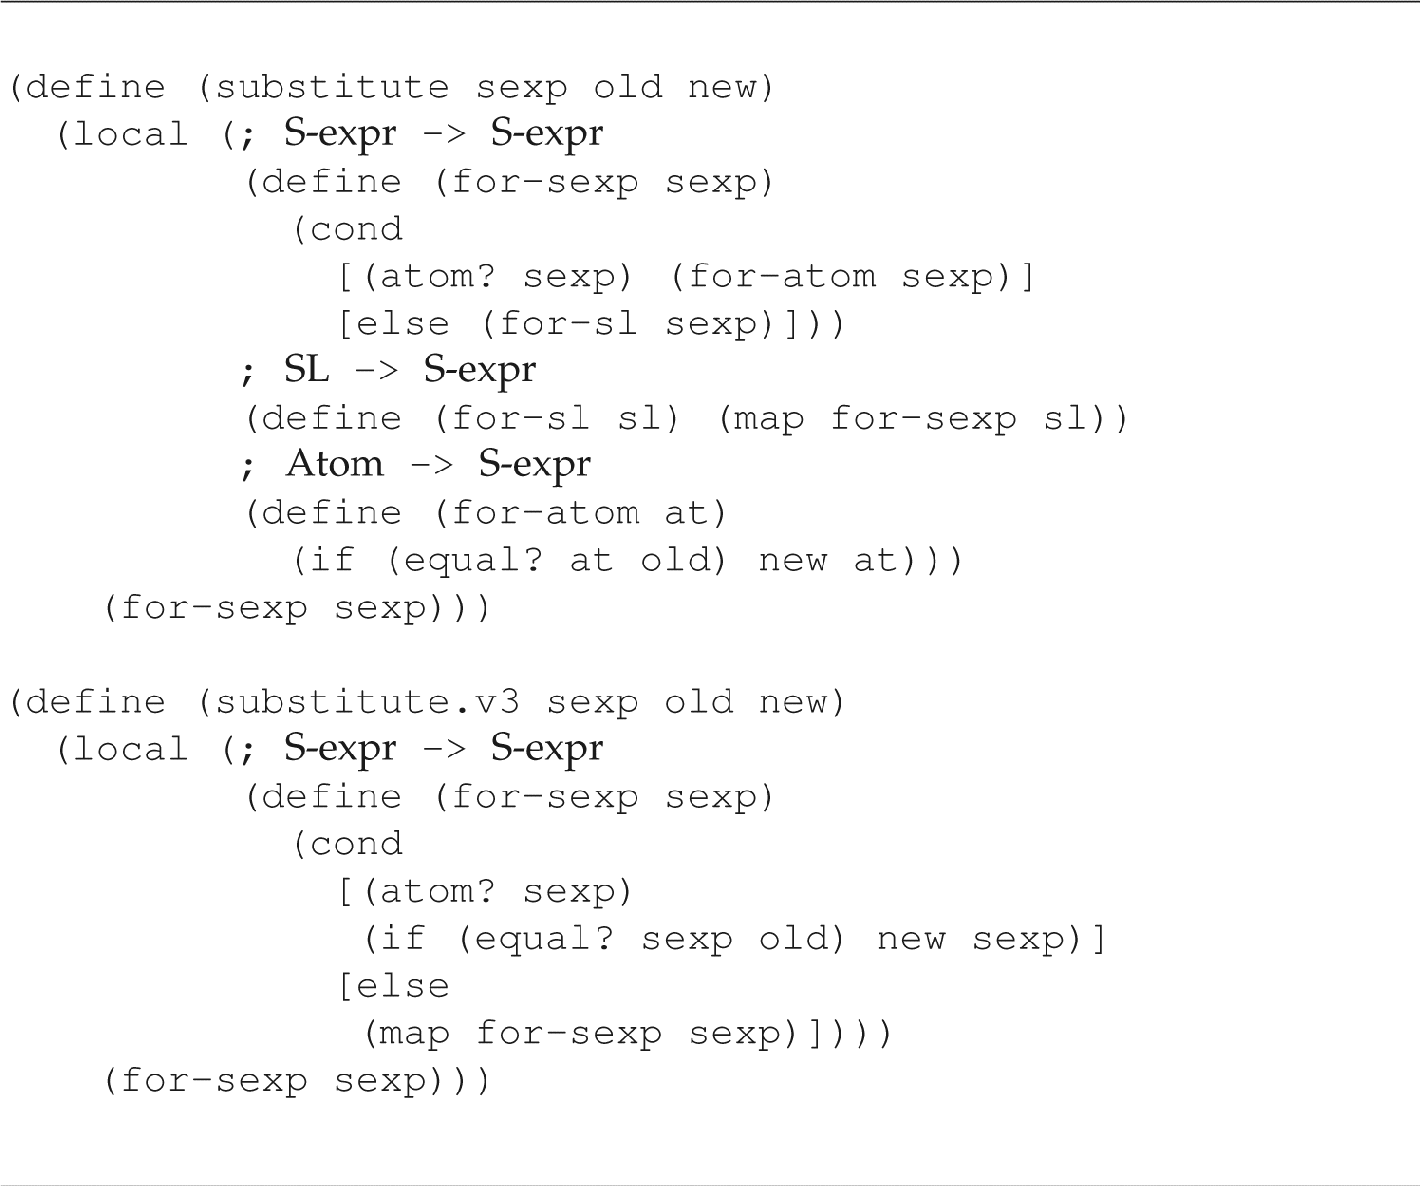
\includegraphics[width=0.85\textwidth]{images/00479.png}
  \caption{程序化简第二与第三步 (Program simplification, steps 2 and 3)}
  \label{fig:122}
\end{figure}

\textbf{第三步化简：函数内联与 lambda。} 此时，最后两个局部定义都只有一行代码，且两者都不包含递归。因此，我们可以将它们直接\term{内联}（in-line）到 \code{for-sexp} 中：将 \code{(for-atom sexp)} 替换为 \code{(if (equal? sexp old) new sexp)}；对于 \code{(for-sl sexp)}，直接替换为 \code{(map for-sexp sexp)}。

经过这一系列内联与提炼，整个程序最终可以优雅地浓缩为一个高度精炼的单函数结构：

\begin{lstlisting}[language=BSL]
; S-expr Symbol Symbol -> S-expr
; 将 sexp 中所有出现的 old 替换为 new
(define (substitute sexp old new)
  (cond
    [(atom? sexp) (if (equal? sexp old) new sexp)]
    [else
     (map (lambda (s) (substitute s old new)) sexp)]))
\end{lstlisting}

观察上述最终形态：原本三个互递归函数、数十行样板代码，最终化为如此清澈、兼具表现力与数学美感的五行定义。这就是掌握交织数据与高阶抽象后的程序之美！
